\documentclass[10pt]{beamer}
\usepackage{kotex}
\usepackage{commath}
\usepackage{multirow}
\usepackage{multicol}
\usepackage{arydshln} % Include this package
\usepackage{bbding}

\usepackage{tikz}
\usepackage{tikz-cd}
\usetikzlibrary{math} % for calculations
\usetikzlibrary{shapes, arrows.meta, positioning, shadows}
\usetikzlibrary{arrows,shapes.geometric}  % Optional, based on your needs
\usetikzlibrary{3d, calc}
\usetikzlibrary{matrix, positioning, arrows.meta, shapes.multipart, chains}
\usetikzlibrary{decorations.pathreplacing,calligraphy}
\usetheme[progressbar=frametitle]{metropolis}
\usepackage{appendixnumberbeamer}

\usepackage{adjustbox}
\usepackage{booktabs}
\usepackage[scale=2]{ccicons}

\usepackage{tcolorbox}

\usepackage{pgfplots}
\usepgfplotslibrary{fillbetween}
\pgfplotsset{compat=1.15}
\usepgfplotslibrary{dateplot}

\usepackage{xspace}
\newcommand{\themename}{\textbf{\textsc{metropolis}}\xspace}

\usepackage[linesnumbered,ruled]{algorithm2e}
\usepackage{algpseudocode}
\usepackage{setspace}
\SetKwComment{Comment}{/* }{ */}
\SetKwProg{Fn}{Function}{:}{end}
\SetKw{End}{end}
\SetKw{DownTo}{downto}

% Define a new environment for algorithms without line numbers
\newenvironment{algorithm2}[1][]{
	% Save the current state of the algorithm counter
	\newcounter{tempCounter}
	\setcounter{tempCounter}{\value{algocf}}
	% Redefine the algorithm numbering (remove prefix)
	\renewcommand{\thealgocf}{}
	\begin{algorithm}
	}{
	\end{algorithm}
	% Restore the algorithm counter state
	\setcounter{algocf}{\value{tempCounter}}
}

\usepackage{xcolor}   % Required for specifying colors

\usepackage{listings} %Code
\renewcommand{\lstlistingname}{Code}%
\definecolor{keyword}{RGB}{255, 0, 0}
\definecolor{identifier}{RGB}{0, 0, 255}
\definecolor{comment}{RGB}{0, 128, 0}
\definecolor{string}{RGB}{163, 21, 21}

\lstdefinestyle{c}{
	language=C,
	basicstyle=\ttfamily\small,
	keywordstyle=\color{keyword},
	identifierstyle=\color{identifier},
	commentstyle=\color{comment}\itshape,
	stringstyle=\color{string},
	showstringspaces=false,
	%	numberstyle=\tiny\color{gray},
	%	numbersep=5pt,
	frame=single,
	tabsize=4,
	captionpos=b,
	breaklines=true,
	breakatwhitespace=true,
	%	numbers=left
}

\usepackage{amsthm, amsmath}


\newcommand{\cyclic}[1]{\langle #1 \rangle}
\newcommand{\uniform}{\overset{\$}{\leftarrow}}
\newcommand{\N}{\mathbb{N}}
\newcommand{\Z}{\mathbb{Z}}
\newcommand{\Q}{\mathbb{Q}}
\newcommand{\R}{\mathbb{R}}
\newcommand{\C}{\mathbb{C}}
\newcommand{\F}{\mathbb{F}}

\newcommand{\xmark}{\textcolor{red}{\XSolidBrush}}
\newcommand{\vmark}{\textcolor{green!75!black}{\CheckmarkBold}}

\newcommand{\B}{\mathbb{B}}
\newcommand{\true}{\textcolor{red}{\texttt 1}}
\newcommand{\false}{\textcolor{red}{\texttt 0}}
\newcommand{\id}{\textnormal{id}}
\title{\huge\bf Software Verification}
\subtitle{\textcolor{magenta}{\textbf{Lecture 02. OCaml Programming II}}}
% \date{\today}
\date{}
\author{\large\textcolor{cyan}{\bf Ji, Yong-Hyeon}\\ \\ \small 24. 07. 25 (Thu)}
\institute{\small
	Coding \& Optimization Together (CO2) \\
	Crypto \& Security Engineering Lab (CSE) \\
	Department of Information Security, Cryptology, and Mathematics
}
% \titlegraphic{\hfill\includegraphics[height=1.5cm]{logo.pdf}}

\begin{document}
	
	\maketitle
	
	\begin{frame}{Table of Contents}
		\setbeamertemplate{section in toc}[sections numbered]
		\tableofcontents%[hideallsubsections]
	\end{frame}
	
	\section{Solutions for Homework}
	\begin{frame}{1. Motivation}
		\url{https://www.tiobe.com/tiobe-index/}
		\begin{figure}[h!]
			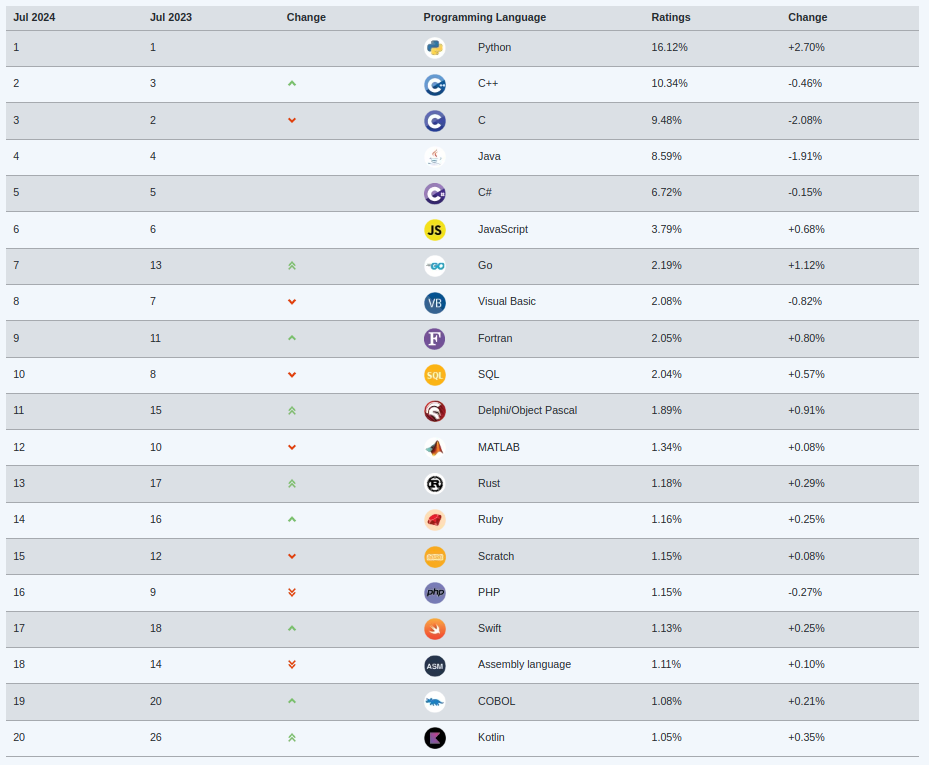
\includegraphics[scale=.35]{ranking1}
		\end{figure}
	\end{frame}
	\begin{frame}{1. Motivation}
	\begin{figure}[h!]
		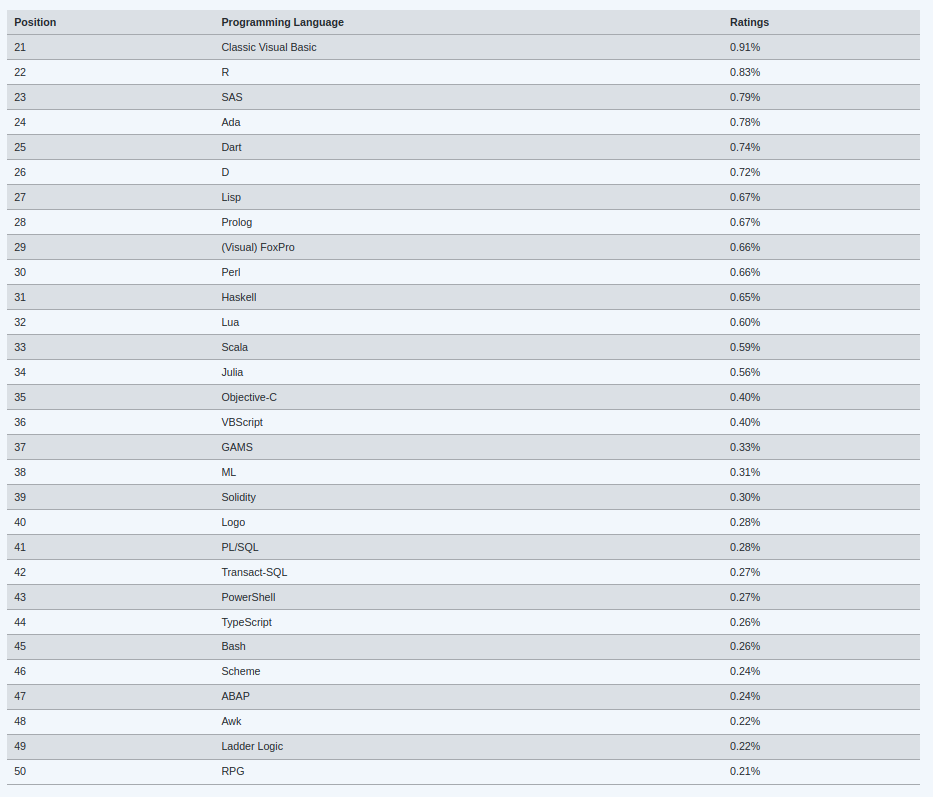
\includegraphics[scale=.35]{ranking2}
	\end{figure}
	\end{frame}
%	\begin{frame}{1. Motivation}
%		\begin{enumerate}
%			\item[3.] Current Technologies for Safe Software
%			\begin{enumerate}[(a)]
%				\item[]
%				\item Code Review
%				\item[]
%				\item Testing
%				\item[]
%				\item Debugging
%				\item[]
%				\item Simulation
%				\item[]
%				\item $\cdots$
%			\end{enumerate}
%		\end{enumerate}
%	\end{frame}

	\section{Basic OCaml Programming}
	\subsection{2.1 OCaml 기본 구성}
	\begin{frame}{2.1 OCaml 기본 구성}
		\textbf{OCaml 프로그램의 기본 단위 공식}
		
		\begin{itemize}
			\item 프로그램을 구성하는 두 가지 기본 단위
			\begin{itemize}
				\item[]
				\item[] Statement: \[
				\texttt{x = x + 1}
				\]
				\item[] Expression: \[
				\texttt{(x + y) * 2}
				\]
			\end{itemize}
		\end{itemize}
	\end{frame}

\begin{lstlisting}[style=ocaml]
let hello = "Hello"
let world = "World"
let helloworld = hello ^ " " ^ world
let _ = print_endline helloworld
\end{lstlisting}

Compile
\begin{lstlisting}[style=zsh]
@:~$>ocaml helloworld.ml
\end{lstlisting}

OCaml REPL(Real-Eval-Print Loop)
\begin{lstlisting}[style=zsh]
@:~$>ocaml

# #use "helloworld.ml";;
val hello : string = "Hello"
val world : string = "World"
val helloworld : string = "Hello World"
Hello World
- : unit = ()
# exit 1;;
\end{lstlisting}
	\newpage
	\begin{frame}{2.1 OCaml 기본 구성}
		\textbf{$\triangleright$ \textcolor{red}{Function Expression} (함수식)}
		\[
		\texttt{fun $x$ -> $e$}
		\] 
		\begin{itemize}
			\item 함수의 예:
			\begin{itemize}
				\item[*] \texttt{fun $x$ -> $x+1$}
				\item[*] \texttt{fun $y$ -> $y*y$}
				\item[*] \texttt{fun $x$ -> if $x>0$ then $x+1$ else $x*x$}
				\item[*] \texttt{fun $x$ -> fun $y$ -> $x+y$}
				\item[*] \texttt{fun $x$ -> fun $y$ -> fun $z$ -> $x+y+z$}
			\end{itemize}
			\item[]
			\item Syntactic Sugar \[
			\texttt{fun $x_1\ \dots\ x_n$\ ->\ $e$}
			\]
			\begin{itemize}
				\item[*] \texttt{fun $x$ $y$ -> $x+y$}
				\item[*] \texttt{fun $x$ $y$ $z$ -> $x+y+z$}
			\end{itemize}
		\end{itemize}
	\end{frame}
	\begin{frame}{2.1 OCaml 기본}
		\textbf{$\triangleright$ Function Call Expression (함수 호출식)} \[
		e_1\quad e_2
		\]
		\begin{tcolorbox}[colback=backcolor]\ttfamily
			\# (fun x -> x * x) 3;;\\
			- : int = 9\\
			\# (fun x -> if x > 0 then x + 1 else x * x) 1;;\\
			- : int = 2\\
			\# (fun x -> fun y -> fun z -> x + y + z) 1 2 3;;\\
			- : int = 6
		\end{tcolorbox}
		
		\begin{tcolorbox}[colback=backcolor]\ttfamily
			\# (fun f -> f * 1) (fun x -> x * x);;\\
			- : int = 1\\
			\# (fun x -> x * x) ((fun x -> if x > 0 then 1 else 2) 3);;\\
			- : int = 2
		\end{tcolorbox}
	\end{frame}

	\begin{frame}{2.1 OCaml 기본}
		\textbf{$\triangleright$ Let Expressions}
		
		값에 이름 붙이기! \[
		\texttt{let}\ x = e_1\ \texttt{in}\ e_2
		\]
		\begin{itemize}
			\item $e_1$의 값을 $x$라고 하고 $e_2$를 계산
			\begin{itemize}
				\item[*] $x$: variable (변수, 값의 이름)
				\item[*] $e_1$: binding expression (정의식)
				\item[*] $e_2$: body expression (몸통식)
			\end{itemize}
			\item $e_2$: scope of $x$ (유효범위)
		\end{itemize}
		 \begin{tcolorbox}[colback=backcolor]\ttfamily
			\# let x = 1 in x + x;;\\
			- : int = 2\\
			\# (let x = 1 in x) + x;;\\
			Error: Unbound value x\\
			\# (let x = 1 in x) + (let x = 2 in x);; \\
			- : int = 3
		\end{tcolorbox}	
		\begin{itemize}
			\item[] 
			\item[] 
			\item[] 
			\item[] 
			\item[] 
		\end{itemize}
	\end{frame}

\begin{lstlisting}[style=zsh]
# let x = (let y = 1 in y + 1) in x + 1;;
- : int = 3
# let x = 1 in
	let y = 2 in
		x + y;;
- : int = 3
\end{lstlisting}

\begin{lstlisting}[style=zsh]
# let square = fun x -> x * x in square 2;;
- : int = 4
# let add x y = x + y in add 1 2;;
- : int = 3
\end{lstlisting}

\begin{lstlisting}[style=zsh]
# let rec factorial n =
	if n = 0 then 1
	else n * factorial (n - 1);;    
val factorial : int -> int = <fun>
# factorial 5;;
- : int = 120
\end{lstlisting}
	\newpage
	\begin{frame}{2.1 OCaml 기본}
		\textbf{$\triangleright$ Pattern Matching (패턴 매칭)}
		
		\begin{itemize}
			\item 패턴 매칭을 이용한 값의 구조 분석
		\end{itemize}
		\begin{tcolorbox}[colback=backcolor]\ttfamily
		\# let rec factorial n =\\
			if n = 0 then 1 else n * factorial (n - 1);; \\   
		val factorial : int -> int = <fun>
		\end{tcolorbox}
		\begin{tcolorbox}[colback=backcolor]\ttfamily
			\# let factorial a = \\
			match a with\\
			0 -> 1\\
			|\_ -> a * factorial (a-1);;\\
			val factorial : int -> int = <fun>
		\end{tcolorbox}
		\begin{itemize}
			\item[]
			\item[]
		\end{itemize}
	\end{frame}

	\begin{frame}{2.1 OCaml 기본}
		\textbf{$\triangleright$ Polymorphic Type (다형 타입)}
		
		\begin{tcolorbox}[colback=backcolor]\ttfamily
			\# let id x = x;; \\
			val id : 'a -> 'a = <fun> \\
			\# id 1;; \\
			- : int = 1 \\
			\# id "abc";; \\
			- : string = "abc" \\
			\# id true;; \\
			- : bool = true \\
		\end{tcolorbox}
		\begin{itemize}
			\item[]
			\item[]
		\end{itemize}
	\end{frame}

	\begin{frame}{2.1 OCaml 기본 구성}
		\textbf{$\triangleright$ Boolean Expressions (논리식)}
		
		\begin{itemize}
			\item 논리값
		\end{itemize}
		\begin{tcolorbox}[colback=backcolor]\ttfamily
			\# true;; \\
			- : bool = true\\
			\# false;; \\
			- : bool = false
		\end{tcolorbox}
		\begin{itemize}
			\item 비교 연산자 (산술식 $\to$ 논리식)
		\end{itemize}
		\begin{tcolorbox}[colback=backcolor]\ttfamily
			\# 1 = 2;; \\
			- : bool = false\\
			\# 1 <> 2;; \\
			- : bool = true\\
			\# 2 <= 2;; \\
			- : bool = true
		\end{tcolorbox}
	\end{frame}

	\begin{frame}{2.1 OCaml 기본 구성}
		\textbf{$\triangleright$ Boolean Expressions (논리식)}
		
		\begin{itemize}
			\item 논리 연산자 (논리식 $\to$ 논리식)
		\end{itemize}
		\begin{tcolorbox}[colback=backcolor]\ttfamily
			\# true \&\& (false || not false);; \\
			- : bool = true\\
			\# (2 > 1) \&\& (3 > 2);; \\
			- : bool = false
		\end{tcolorbox}
		\begin{itemize}
			\item[] 
			\item[] 
			\item[] 
			\item[] 
			\item[] 
			\item[] 
			\item[] 
		\end{itemize}
	\end{frame}

	\begin{frame}{2.1 OCaml 기본 구성}
		\textbf{$\triangleright$ Primitive Values (기본값)}
		
		\begin{itemize}
			\item OCmal은 \begin{itemize}
				\item[-] integer (정수) 
				\item[-] float (실수)
				\item[-] boolean (논리)
				\item[-] character (문자)
				\item[-] string (문자열)
				\item[-] unit (유닛)
			\end{itemize}을 제공
		\end{itemize}
		\begin{tcolorbox}[colback=backcolor]\ttfamily
			\# 'c';; \\
			- : char = 'c'\\
			\# "Objecive " \^{} "Caml";; \\
			- : string = "Objective Caml"\\
			\# ();;\\
			- : unit = ()
		\end{tcolorbox}
	\end{frame}

	\begin{frame}{2.1 OCaml 기본 구성}
		\textbf{$\triangleright$ Conditional Expression (조건식)}	
		\[
		\texttt{if $e_1$ then $e_2$ else $e_3$}
		\]
		\begin{tcolorbox}[colback=backcolor]\ttfamily
		\# if 1 then 2 else 3;;
		\end{tcolorbox}
		\begin{itemize}
			\item[] 
			\item[] 
			\item[] 
			\item[] 
			\item[] 
			\item[] 
			\item[] 
			\item[] 
		\end{itemize}
	\end{frame}
	\begin{frame}{2.1 OCaml 기본 구성}
		\textbf{$\triangleright$ Conditional Expression (조건식)}	
		\[
		\texttt{if $e_1$ then $e_2$ else $e_3$}
		\]
		\begin{itemize}
			\item $e_1$은 반드시 논리식이어야 함. 즉 $e_1$의 값은 true or false
		\end{itemize}
		\begin{tcolorbox}[colback=backcolor]\ttfamily
			\# if 1 then 2 else 3;;\\
			Error: This expression has type int but an expression was expected of type
			bool
			because it is in the condition of an if-statement
		\end{tcolorbox}
		\begin{itemize}
			\item[] 
			\item[] 
			\item[] 
		\end{itemize}
	\end{frame}
	
	\begin{frame}{2.1 OCaml 기본 구성}
		\textbf{$\triangleright$ Conditional Expression (조건식)}
		\begin{itemize}
			\item 조건식의 값은 $e_1$ 값에 따라서 결정
		\end{itemize}
		\begin{tcolorbox}[colback=backcolor]\ttfamily
			\# if 2 $>$ 1 then 0 else 1;;\\
			- : int = 0 \\
			\# if 2 < 1 then 0 else 1;; \\
			- : int = 1
		\end{tcolorbox}
		\begin{itemize}
			\item $e_2$와 $e_3$는 타입이 같아야 함
		\end{itemize}
		\begin{tcolorbox}[colback=backcolor]\ttfamily
			\# if true then 1 else true;;\\
			Error: This expression has type bool but an expression was expected of type
			int
		\end{tcolorbox}
		\begin{itemize}
			\item[]
		\end{itemize}
	\end{frame}

	\begin{frame}{2.1 OCaml 기본 구성}
		\textbf{$\triangleright$ \textcolor{red}{Function Expression} (함수식)}
		\[
		\texttt{fun $x$ -> $e$}
		\] 
		\begin{itemize}
			\item 함수의 예:
			\begin{itemize}
				\item[*] \texttt{fun $x$ -> $x+1$}
				\item[*] \texttt{fun $y$ -> $y*y$}
				\item[*] \texttt{fun $x$ -> if $x>0$ then $x+1$ else $x*x$}
				\item[*] \texttt{fun $x$ -> fun $y$ -> $x+y$}
				\item[*] \texttt{fun $x$ -> fun $y$ -> fun $z$ -> $x+y+z$}
			\end{itemize}
			\item[]
			\item Syntactic Sugar \[
			\texttt{fun $x_1\ \dots\ x_n$\ ->\ $e$}
			\]
			\begin{itemize}
				\item[*] \texttt{fun $x$ $y$ -> $x+y$}
				\item[*] \texttt{fun $x$ $y$ $z$ -> $x+y+z$}
			\end{itemize}
		\end{itemize}
	\end{frame}
\begin{itemize}
	\item[]
	\item[]
	\item[]
\end{itemize}
\begin{lstlisting}[style=zsh]
@:~$>ocaml

# let f = fun x y -> x + y;;
val f : int -> int -> int = <fun>
# f 1 2;
- : int = 3
# let g = f 1;
# g 2;;
- : int = 3
\end{lstlisting}

\newpage
%	\subsection{2.2 리스트와 재귀함수}
%	\begin{frame}{2.2 리스트와 재귀함수}
%		content...
%	\end{frame}
%
%	
%	\subsection{2.3 고차 함수}
%	\begin{frame}{2.3 고차 함수}
%		content...
%	\end{frame}
%	
%	
%	\subsection{2.4 사용자 정의 타입}
%	\begin{frame}{2.4 사용자 정의 타입}
%		content...
%	\end{frame}

	\section{Advanced OCaml Programming}
	
	\newpage
	{\setbeamercolor{palette primary}{fg=black, bg=-blue}
		\begin{frame}[standout]
			To be continue ...
		\end{frame}
	}
	
	%\appendix
	%
	%\begin{frame}[fragile]{Backup slides}
	%  Sometimes, it is useful to add slides at the end of your presentation to
	%  refer to during audience questions.
	%
	%  The best way to do this is to include the \verb|appendixnumberbeamer|
	%  package in your preamble and call \verb|\appendix| before your backup slides.
	%
	%  \themename will automatically turn off slide numbering and progress bars for
	%  slides in the appendix.
	%\end{frame}
	%
	%\begin{frame}[allowframebreaks]{References}
	%
	%  \bibliography{demo}
	%  \bibliographystyl{abbrv}
	%
	%\end{frame}
	
\end{document}
